\section{OpenCV}

\begin{frame}{OpenCV}
    Was ist OpenCV?
   \begin{itemize}
   \item OpenCV ist eine plattformübergreifende Bibliothek, für Echtzeit-Computer-Vision-Anwendungen
   \item beinhaltet Algorithmen für die Bildverarbeitung und im Rahmen von Computer Vision (CV) auch für maschinelles Lernen
    \end{itemize}
    
   Wofür nutzen wir OpenCV?
   \begin{itemize}
   \item Nutzung für die Verarbeitung des erkannten Nummernschildes (z.B. Tresholding), um die Zeichen besser zu erkennen und richtig auszulesen
   
   \end{itemize}
\end{frame}

\begin{frame}{Beispiel für die Anwendung von OpenCV}

OpenCV wurde bereits auf Nummernschildverarbeitung verwendet:
\begin{figure}
\begin{center}
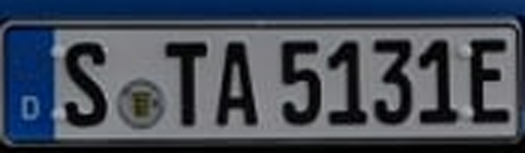
\includegraphics[scale=0.25]{bilder/Nummer_1.png}
\caption{Original}
\label{Original}
\end{center}
\end{figure}

\begin{figure}
\begin{center}
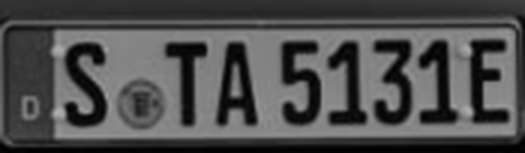
\includegraphics[scale=0.25]{bilder/Nummer_2_grau.png}
\caption{Graustufen}
\label{Graustufen}
\end{center}
\end{figure}

\end{frame}

\begin{frame}{Beispiel für die Anwendung von OpenCV}

\begin{figure}
\begin{center}

\includegraphics[scale=0.25]{bilder/Nummer_3_treshold.png}
\caption{Tresholding}
\label{Tresholding}
\end{center}
\end{figure}

\begin{figure}
\begin{center}
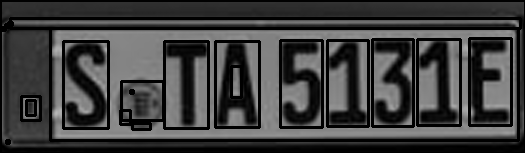
\includegraphics[scale=0.25]{bilder/Nummer_4_Konturen.png}
\caption{Konturen}
\label{Konturen}
\end{center}
\end{figure}

\end{frame}

\begin{frame}{Beispiel für die Anwendung von OpenCV}

\begin{figure}
\begin{center}
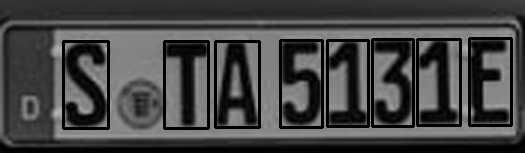
\includegraphics[scale=0.25]{bilder/Nummer_5_Aussortieren.png}
\caption{Aussortierung}
\label{Aussortierung}
\end{center}
\end{figure}

\begin{figure}
\begin{center}
\includegraphics[scale=0.25]{bilder/Nummer_6_SchwarzWeiß.png}
\caption{Schwarze Schrift auf weissem Hintergrund}
\label{SchwarzWeiss}
\end{center}
\end{figure}

Auf das finale Bild (Abbildung 7) wird anschliessend Tesseract angewendet, das die Nummern und Buchstaben ausgibt
\end{frame}